\documentclass[12pt]{article}
\usepackage[T1]{fontenc}
\usepackage[T1]{polski}
\usepackage[utf8]{inputenc}
\usepackage{graphicx}
\usepackage{amsfonts}
\usepackage{float}

\setlength{\textheight}{20cm}

\title{{\bf Zadanie nr 2 - Próbkowanie i kwantyzacja}\linebreak
Cyfrowe Przetwarzanie Sygnałów}
\author{Krzysztof Barden, 210139 \and Paweł Galewicz, 210182}
\date{17.04.2019r.}

\begin{document}
\clearpage\maketitle
\thispagestyle{empty}
\newpage
\setcounter{page}{1}
\section{Cel zadania}

Celem ćwiczenia jest zapoznanie się z praktycznymi aspektami procesu konwersji
analogowo-cyfrowej (A/C) i cyfrowo-analogowej (C/A) sygnałów.. Zostały wykonane następujące warianty:

\begin{itemize}
\item (S1) Próbkowanie równomierne,
\item (Q1) Kwantyzacja równomierna z obcięciem,
\item (R2) Interpolacja pierwszego rzędu,
\item (R3) Rekonstrukcja w oparciu o funkcję sinc.
\end{itemize}

Program wylicza też następujące dodatkowe parametry sygnału:
\begin{itemize}
\item Błąd sreniokwadratowy (MSE), 
\item Stosunek sygnał - szum (SNR), 
\item Szczytowy stosunek sygnał - szum (PSNR), 
\item Maksymalna różnica (MD), 
\item Efektywna liczba bitów (ENOB).
\end{itemize}

\section{Wstęp teoretyczny}

Program z zadania 1 został rozszerzony o dodadtkowe funkcjonalnosci. Wykresy generowane są przy użyciu biblioteki LiveCharts \cite{lv}. GUI aplikacji zostało stworzone przy użyciu biblioteki WPF \cite{wpf}.
\\Po włączeniu się programu pojawia się dany interfejs:
\begin{figure}[H]
 \centering
 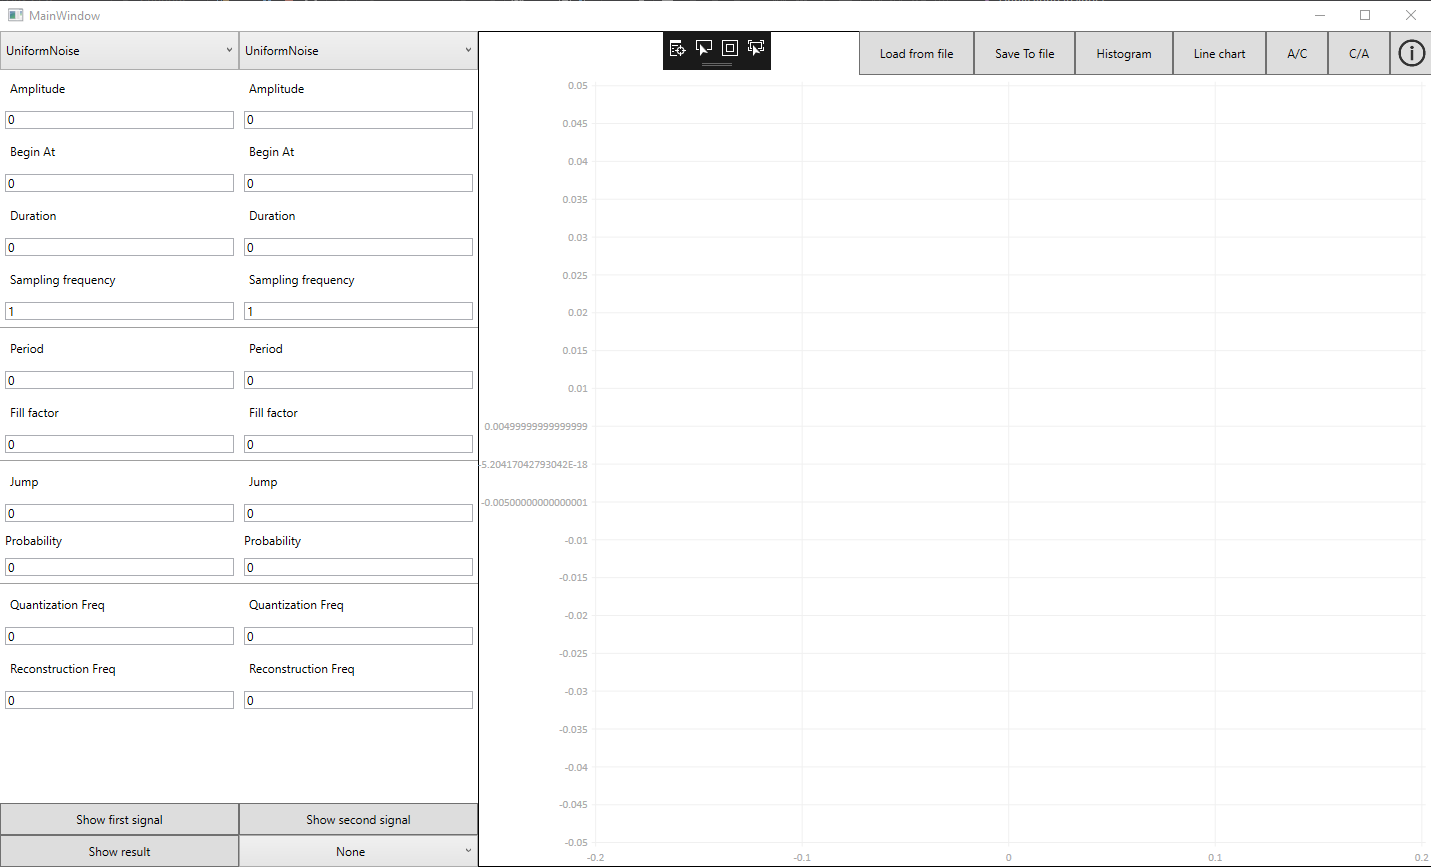
\includegraphics[width=15cm]{images/gui1.PNG}
 \vspace{-0.3cm}
 \caption{Interfejs graficzny użytkownika}
 \label{gui}
\end{figure}

Aby wygenerować sygnał należy w lewej kolumnie wybrać z listy odpowiedni rodzaj sygnału,  wypełnić parametry i nacisnąć przycisk "Show first signal". Aby wygenerować sygnały powstałe przy konwersji A/C należy nacisnąć przycisk "A/C", a by  wygenerować sygnały powstałe przy konwersji C/A należy nacisnąć przycisk "C/A"

Aby wyswietlić obliczone wartosci należy nacisnąć przycisk w prawym górnym rogu ('i' w kółku).
\section{Eksperymenty i wyniki}


%%%%%%%%%%%%%%%%%%%%%%%%%%%%%%%%%%%%%%%%%%%%%%%%%%%%%%%%%%%%%%%%%%%%%%%%%%%%%%%%%%%%%%%%%%%%%%%%%%%%%%%%%%%%%%%%%
% PODROZDZIAŁ PT. EKSPERYMENT NR 1 
%%%%%%%%%%%%%%%%%%%%%%%%%%%%%%%%%%%%%%%%%%%%%%%%%%%%%%%%%%%%%%%%%%%%%%%%%%%%%%%%%%%%%%%%%%%%%%%%%%%%%%%%%%%%%%%%%

Do zaprezentowania możliwosci programu przedstawimy 3 esperymenty:
\begin{itemize}
\item Generowanie szumu o rozkladzie jednostajnym;
\item Generowanie sygnału sinusoidalnego wyprostowanego jednopołówkowo;
\item Suma sygnału trójkątnego i szumu gaussowskiego;
\end{itemize}


\subsection{Eksperyment nr 1 }
\subsubsection{Generowanie szumu o rozkladzie jednostajnym}
Celem tego eksperymentu było wygenerowanie szumu o rozkladzie jednostajnym.


\subsubsection{Rezultat}

\begin{figure}[H]
 \centering
 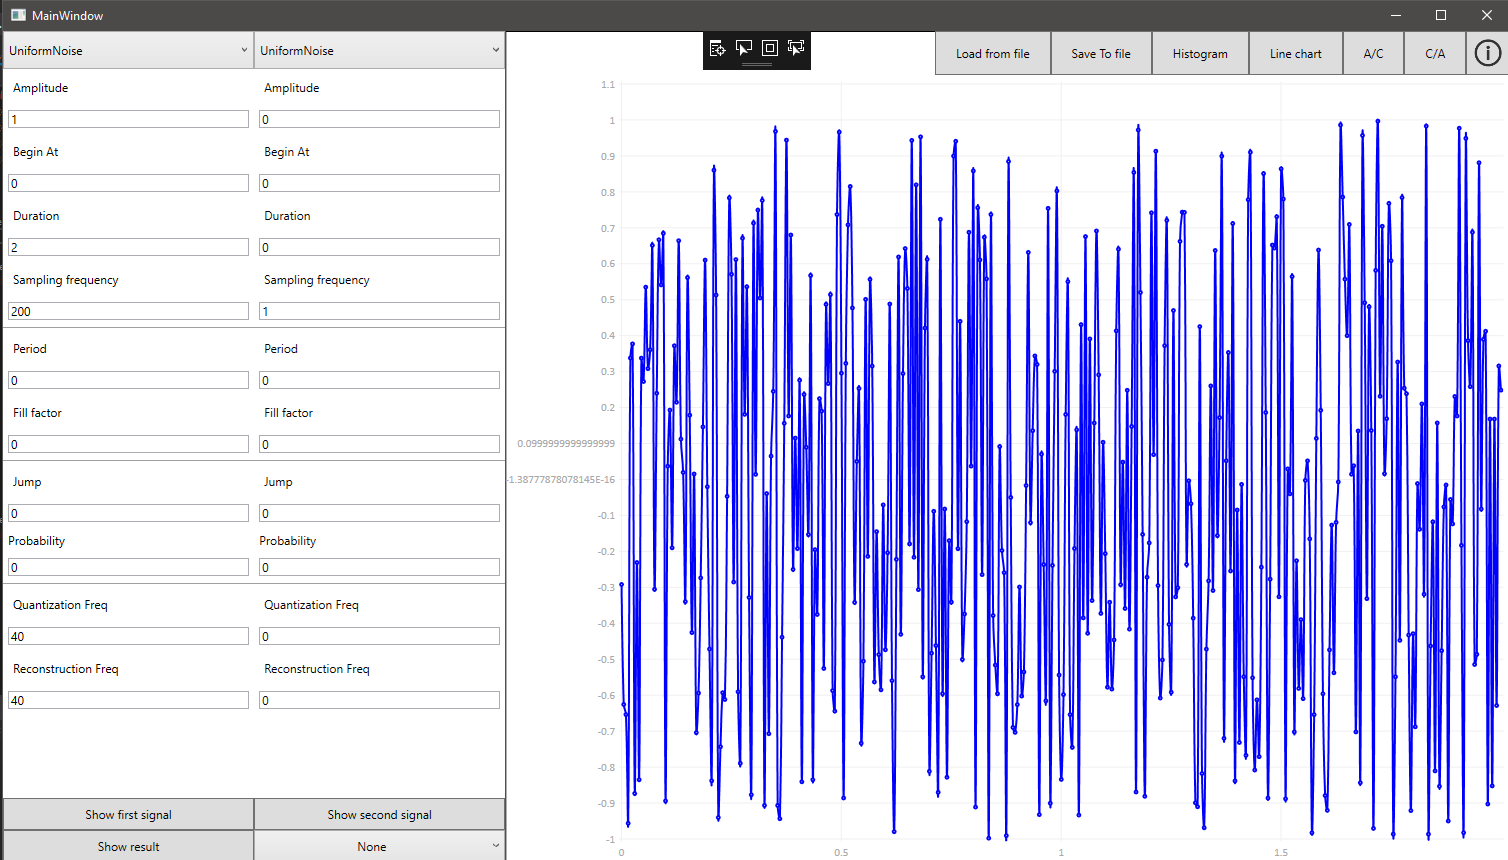
\includegraphics[width=14cm]{images/uniline.PNG}
 \vspace{-0.3cm}
 \caption{Wykres szumu o rozkladzie jednostajnym}
 \label{gui}
\end{figure}

\begin{figure}[H]
 \centering
 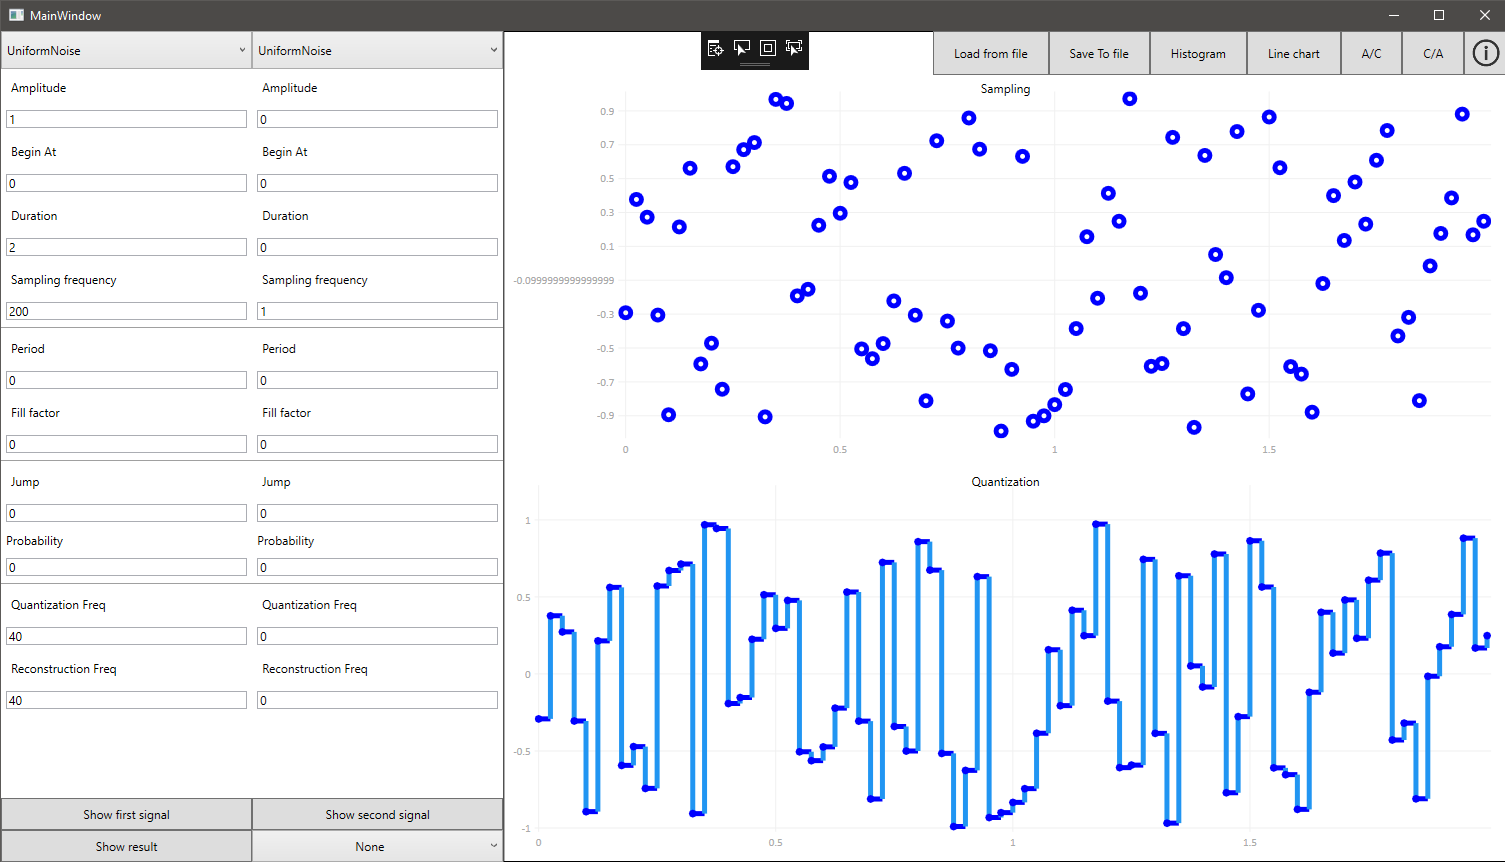
\includegraphics[width=14cm]{images/uniac.PNG}
 \vspace{-0.3cm}
 \caption{Konwersja A/C}
 \label{gui}
\end{figure}

\begin{figure}[H]
 \centering
 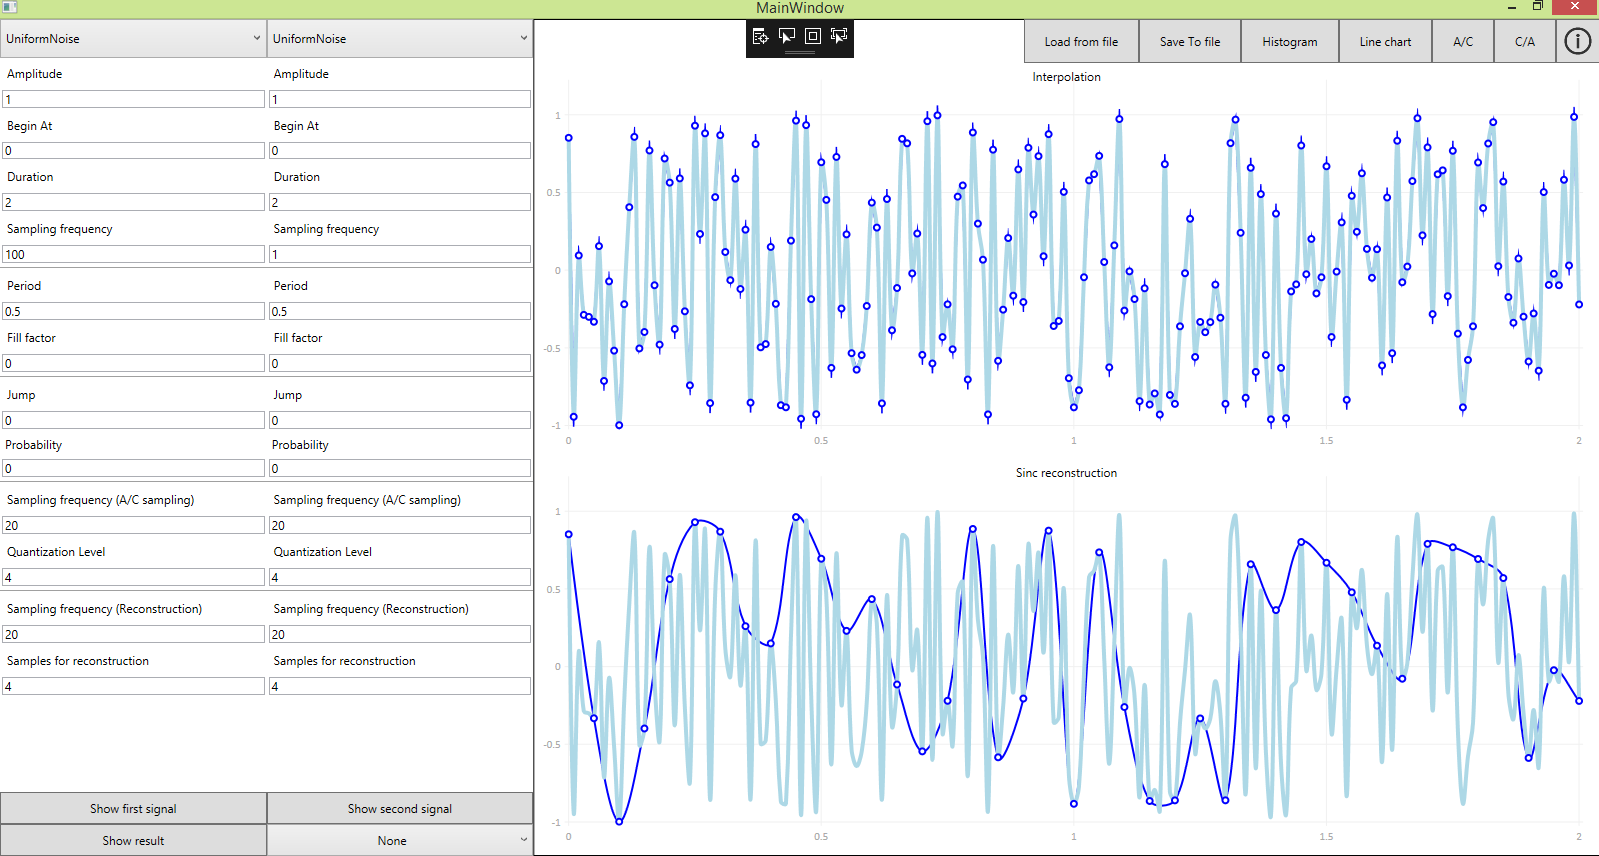
\includegraphics[width=14cm]{images/unica.PNG}
 \vspace{-0.3cm}
 \caption{Konwersja C/A}
 \label{gui}
\end{figure}

\begin{figure}[H]
 \centering
 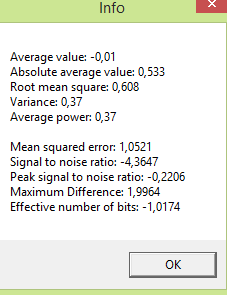
\includegraphics[width=7cm]{images/uniinfo.PNG}
 \vspace{-0.3cm}
 \caption{Wyliczone wartosci dla szumu o rozkladzie jednostajnym}
 \label{gui}
\end{figure}


%%%%%%%%%%%%%%%%%%%%%%%%%%%%%%%%%%%%%%%%%%%%%%%%%%%%%%%%%%%%%%%%%%%%%%%%%%%%%%%%%%%%%%%%%%%%%%%%%%%%%%%%%%%%%%%%%
% PODROZDZIAŁ PT. EKSPERYMENT NR 2
%%%%%%%%%%%%%%%%%%%%%%%%%%%%%%%%%%%%%%%%%%%%%%%%%%%%%%%%%%%%%%%%%%%%%%%%%%%%%%%%%%%%%%%%%%%%%%%%%%%%%%%%%%%%%%%%%


\subsection{Eksperyment nr 2 }
\subsubsection{Generowanie sygnału sinusoidalnego wyprostowanego jednopołówkowo}
Celem tego eksperymentu było wygenerowanie szumu o rozkladzie jednostajnym.


\subsubsection{Rezultat}

\begin{figure}[H]
 \centering
 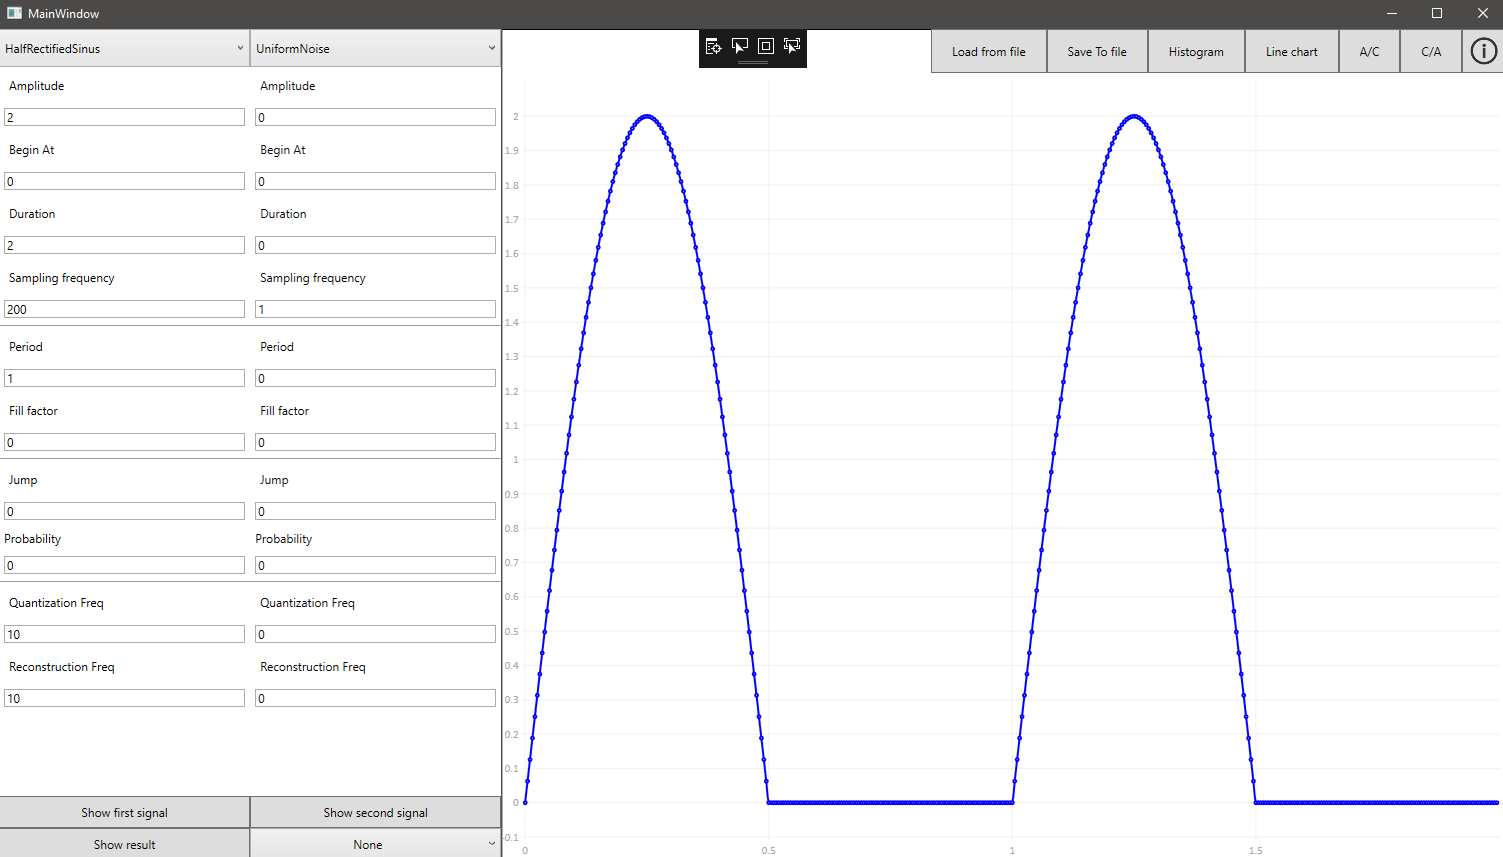
\includegraphics[width=14cm]{images/hsinline.PNG}
 \vspace{-0.3cm}
 \caption{Wykres sygnału sinusoidalnego wyprostowanego jednopołówkowo}
 \label{gui}
\end{figure}

\begin{figure}[H]
 \centering
 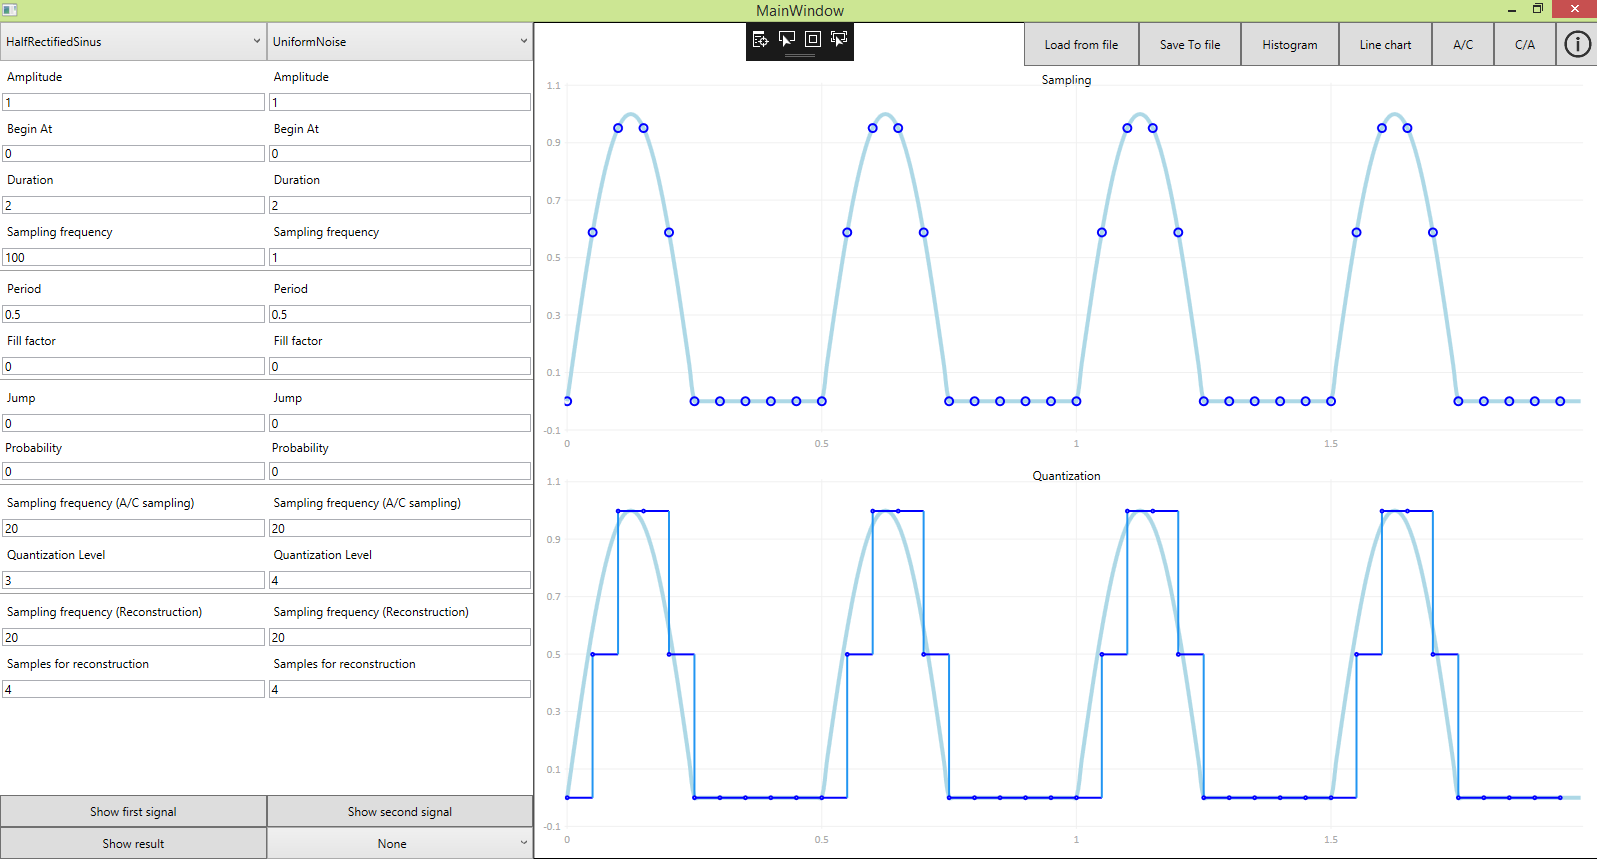
\includegraphics[width=14cm]{images/hsinac.PNG}
 \vspace{-0.3cm}
 \caption{Konwersja A/C}
 \label{gui}
\end{figure}

\begin{figure}[H]
 \centering
 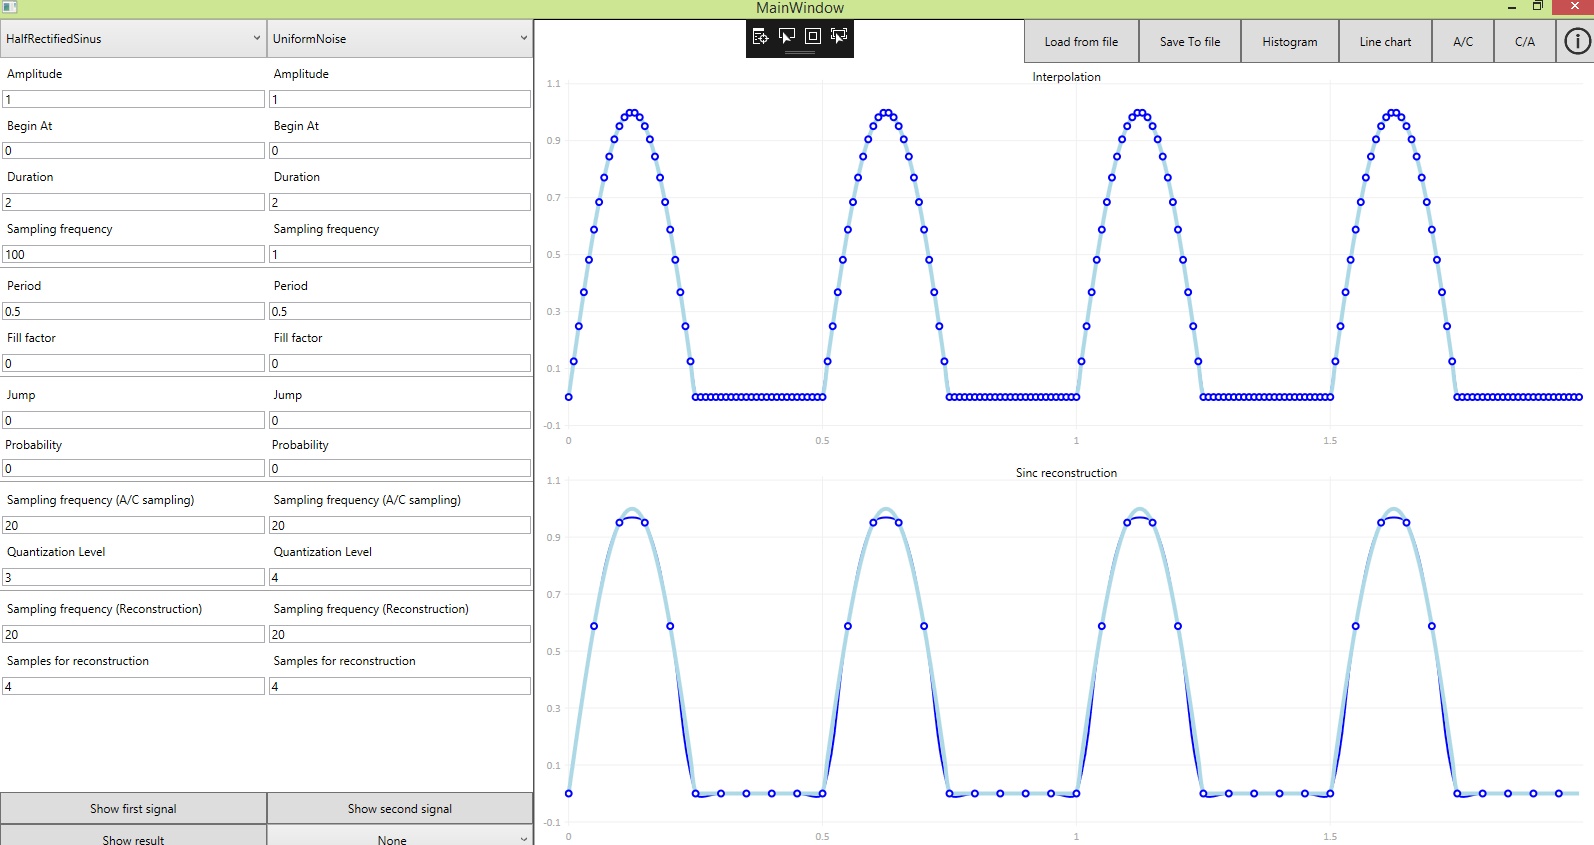
\includegraphics[width=14cm]{images/hsinca.PNG}
 \vspace{-0.3cm}
 \caption{Konwersja C/A}
 \label{gui}
\end{figure}

\begin{figure}[H]
 \centering
 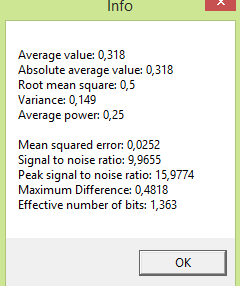
\includegraphics[width=7cm]{images/hsininfo.PNG}
 \vspace{-0.3cm}
 \caption{Wyliczone wartosci dla sygnału sinusoidalnego wyprostowanego jednopołówkowo}
 \label{gui}
\end{figure}



%%%%%%%%%%%%%%%%%%%%%%%%%%%%%%%%%%%%%%%%%%%%%%%%%%%%%%%%%%%%%%%%%%%%%%%%%%%%%%%%%%%%%%%%%%%%%%%%%%%%%%%%%%%%%%%%%
% PODROZDZIAŁ PT. EKSPERYMENT NR 3
%%%%%%%%%%%%%%%%%%%%%%%%%%%%%%%%%%%%%%%%%%%%%%%%%%%%%%%%%%%%%%%%%%%%%%%%%%%%%%%%%%%%%%%%%%%%%%%%%%%%%%%%%%%%%%%%%


\subsection{Eksperyment nr 3 }
\subsubsection{Suma sygnału trójkątnego i szumu gaussowskiego}
Celem tego eksperymentu było wygenerowanie sygnału będącego sumą sygnału trójkątnego i szumu gaussowskiego


\subsubsection{Rezultat}

\begin{figure}[H]
 \centering
 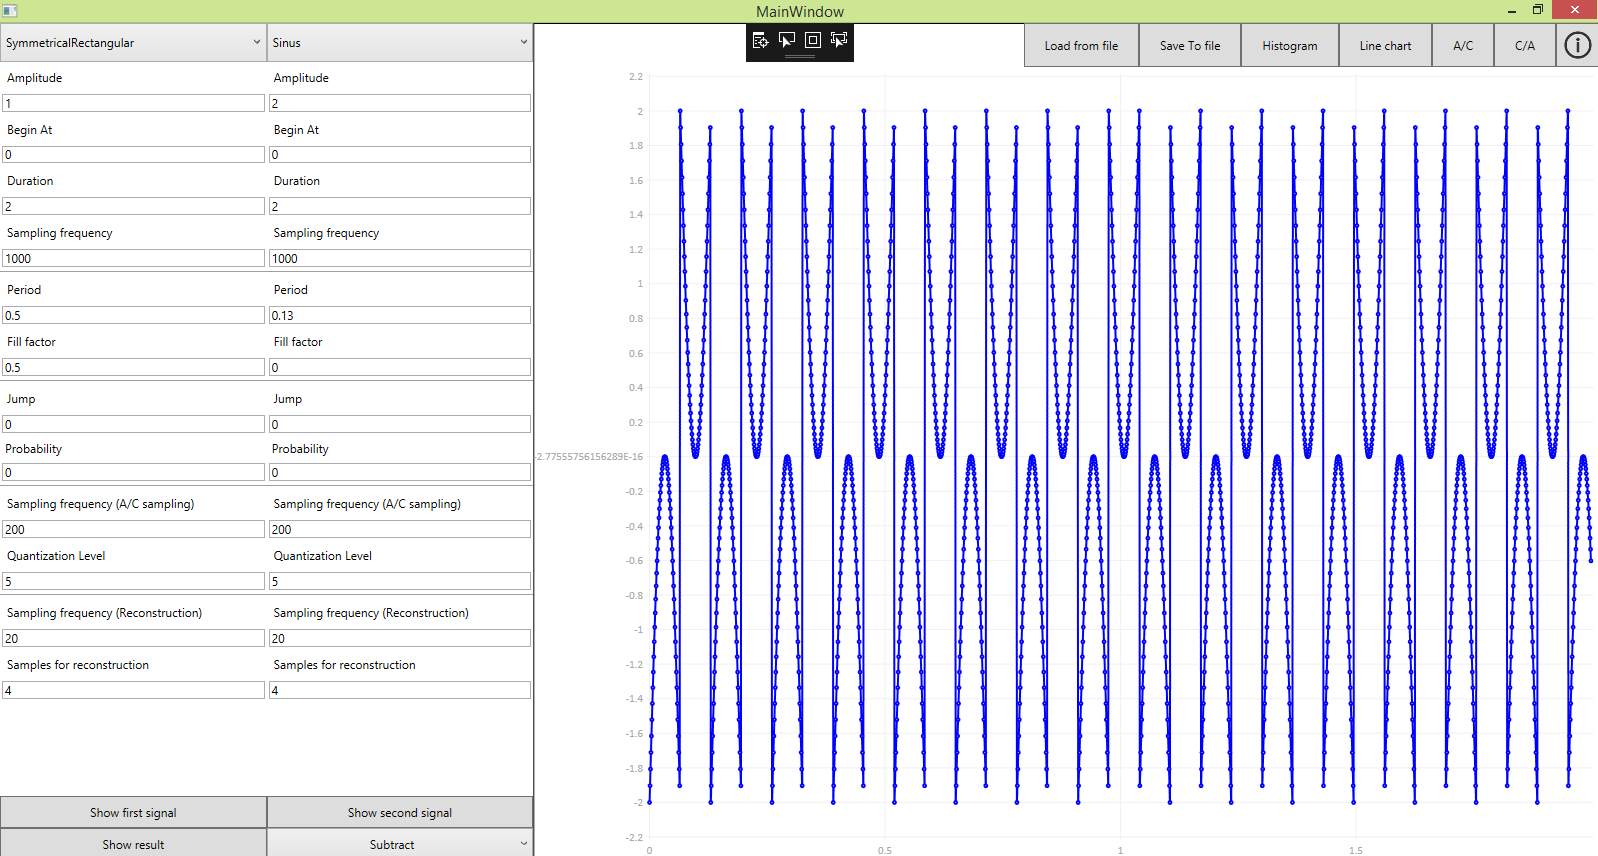
\includegraphics[width=14cm]{images/addline.PNG}
 \vspace{-0.3cm}
 \caption{Wykres sumy sygnału trójkątnego i szumu gaussowskiego}
 \label{gui}
\end{figure}

\begin{figure}[H]
 \centering
 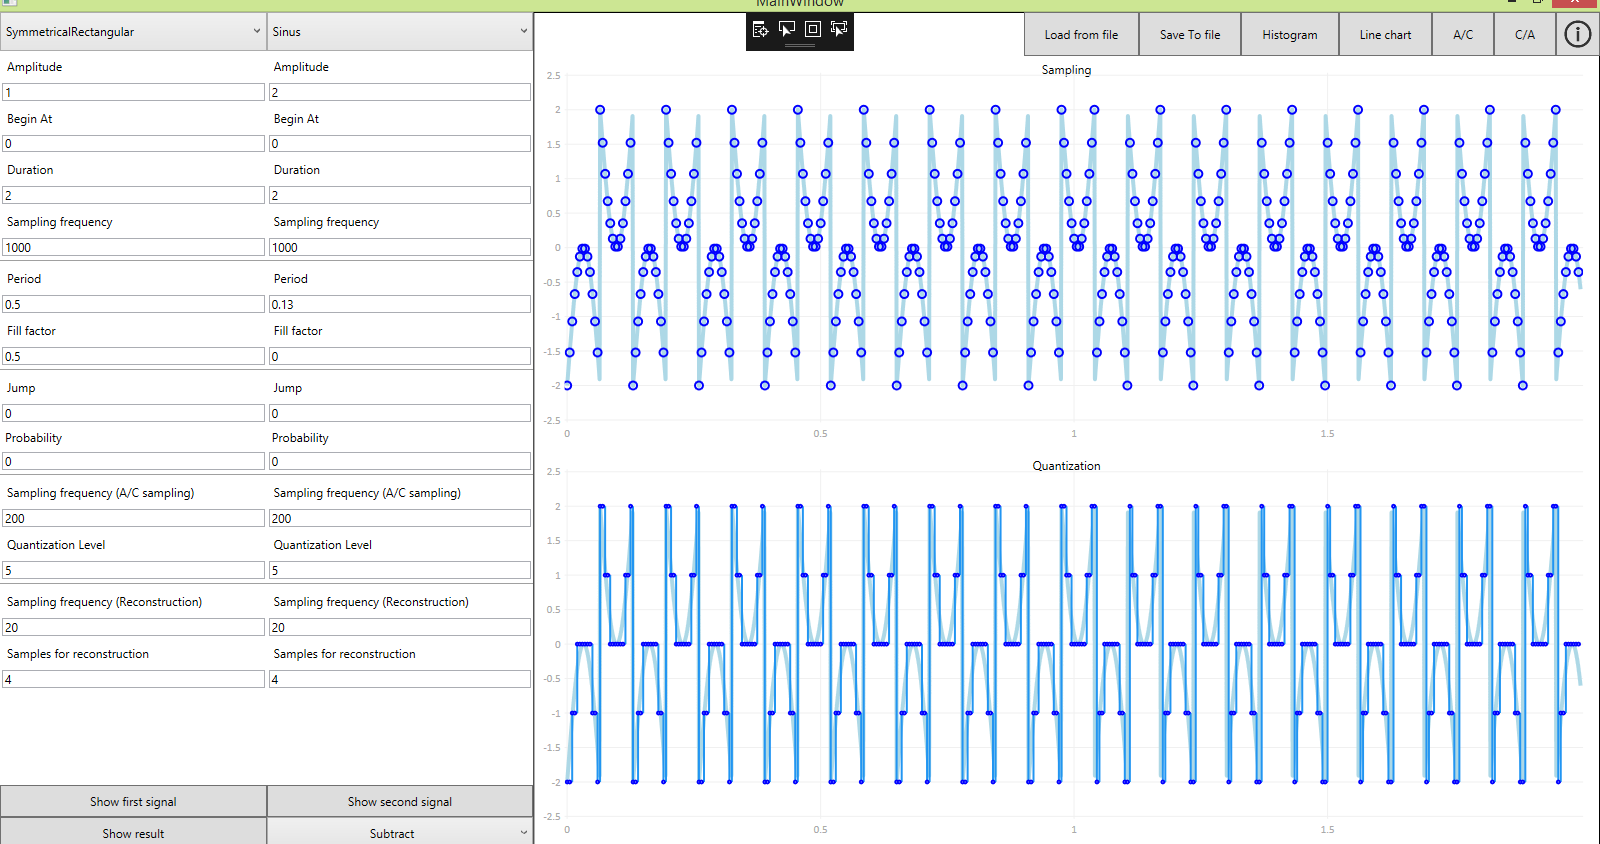
\includegraphics[width=14cm]{images/addac.PNG}
 \vspace{-0.3cm}
 \caption{Konwersja A/C}
 \label{gui}
\end{figure}

\begin{figure}[H]
 \centering
 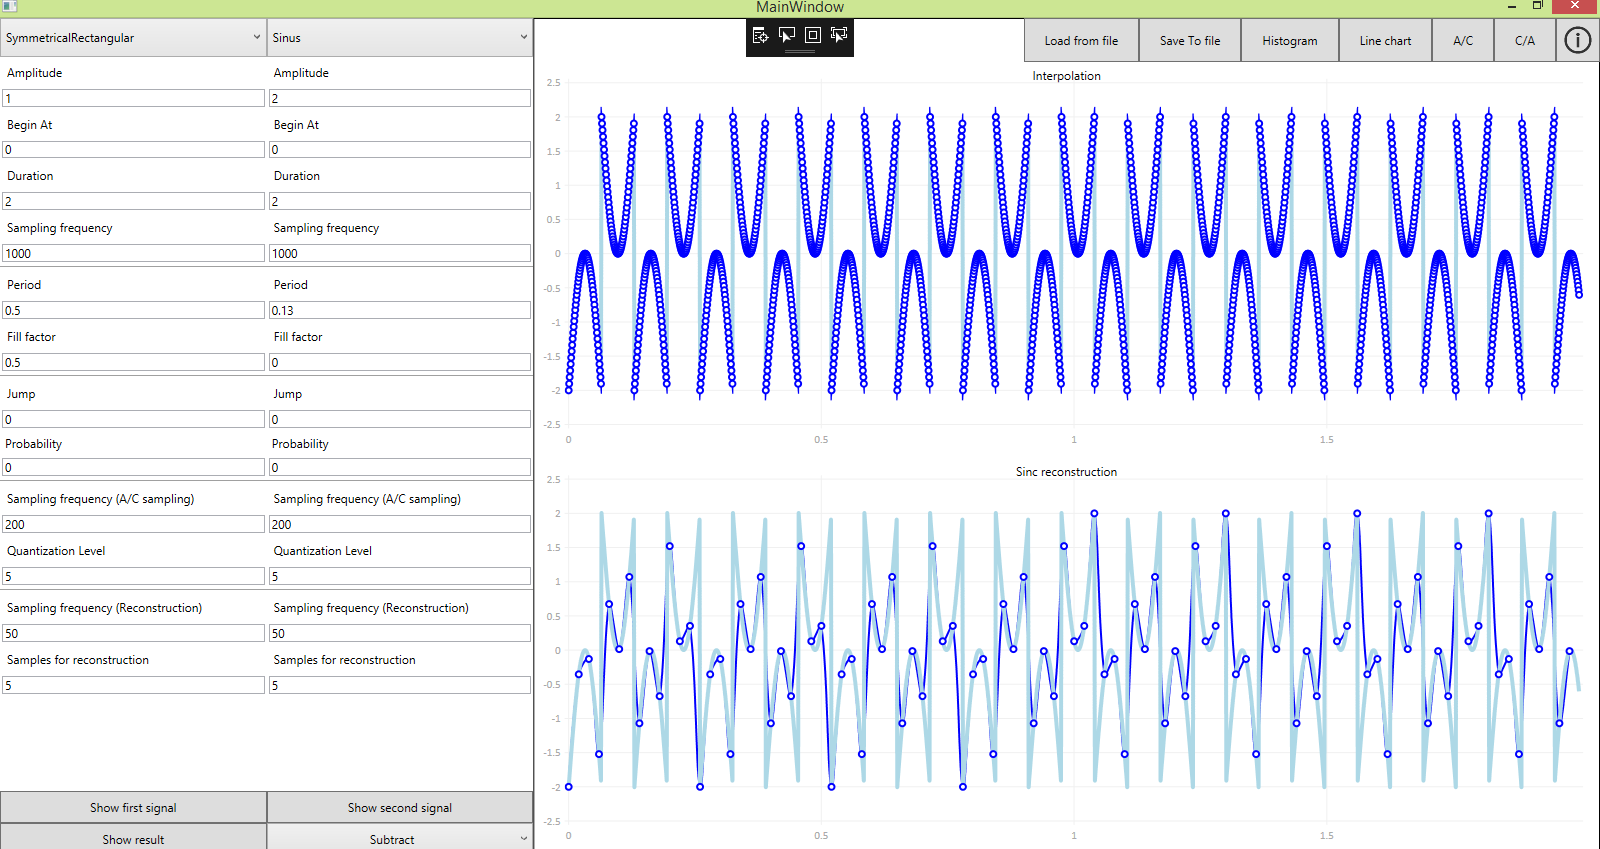
\includegraphics[width=14cm]{images/addca.PNG}
 \vspace{-0.3cm}
 \caption{Konwersja C/A}
 \label{gui}
\end{figure}

\begin{figure}[H]
 \centering
 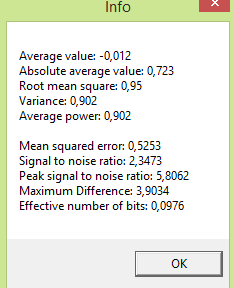
\includegraphics[width=7cm]{images/addinfo.PNG}
 \vspace{-0.3cm}
 \caption{Wyliczone wartosci dla  sumy sygnału trójkątnego i szumu gaussowskiego}
 \label{gui}
\end{figure}




\newpage

\section{Wnioski}

Aplikacja została napisania zgodnie z instrukcją zadania \cite{zad}. Aplikacja pozwala na rozszerzanie jej o kolejne funkcjonalnosci na potrzeby kolejnych zadań. 




%%%%%%%%%%%%%%%%%%%%%%%%%%%%%%%%%%%%%%%%%%%%%%%%%%%%%%%%%%%%%%%%%%%%%%%%%%%%%%%%%%%%%%%%%%%%%%%%%%%%%%%%%%%%%%%%%
% BIBLIOGRAFIA
%%%%%%%%%%%%%%%%%%%%%%%%%%%%%%%%%%%%%%%%%%%%%%%%%%%%%%%%%%%%%%%%%%%%%%%%%%%%%%%%%%%%%%%%%%%%%%%%%%%%%%%%%%%%%%%%%

\begin{thebibliography}{99}
\bibitem{pa} H.~Partl:
\emph{German \TeX},
TUGboat Vol.~9,, No.~1 ('88)
\bibitem{lv} Biblioteka LiveCharts. https://lvcharts.net
\bibitem{wpf} Windows Presentation Foundation. https://docs.microsoft.com/plpl/dotnet/framework/wpf/getting-started/walkthrough-my-frst-wpfdesktop-application
\bibitem{zad} https://ftims.edu.p.lodz.pl/pluginfile.php/13449/mod\_resource/content/0/zadanie2.pdf
\end{thebibliography}

\end{document}
